\section{Analyse de généralisation par ligne de produits logiciels (H4)}
\label{chap:generalisation_spl}

Cette section éprouve la dernière hypothèse, H4 : l'architecture présente un noyau d'invariants stable et des points de variation identifiables, qui permettent de la reprendre dans d'autres PME d'import-export d'Afrique subsaharienne sans refonte majeure. Comme annoncé dans la méthodologie (\S\ref{sec:methodologie}), H4 est éprouvée par le raisonnement et non par la mesure : l'étude de plusieurs cas réels dépassait le temps de ce mémoire.

\subsection{Cadre d'analyse : la SPL appliquée à l'architecture SOYAFF}
\label{sec:spl_cadre}

L'ingénierie des lignes de produits logiciels (\textit{Software Product Lines}, SPL) raisonne sur une famille de systèmes apparentés \cite{clementsSoftwareProductLines2002,fix_pohlSoftwareProductLines2018,apelSoftwareProductLines2013}. Ce qui reste identique d'un produit à l'autre forme le noyau (\textit{commonality}) ; ce qui change est localisé en des points de variation, chacun résolu par le choix d'une variante. Le modèle de caractéristiques (\textit{feature model}) représente cette analyse sous forme d'arbre, et le \textit{binding time} indique à quel moment chaque variation est résolue : à la conception, au déploiement ou à l'exécution.

SOYAFF est traité ici comme le premier produit d'une ligne visant les PME d'import-export d'un corridor transfrontalier, soumises aux contraintes de budget, de connectivité et de souveraineté décrites au chapitre~\ref{chap:contexte}. L'analyse part de l'architecture réellement construite (section~\ref{chap:architecture} et chapitre~\ref{chap:realisation}). Elle établit la \emph{plausibilité} de H4, pas sa validation.

\subsection{Le noyau invariant}
\label{sec:spl_invariants}

Six invariants se dégagent de l'architecture (Tableau~\ref{tab:invariants_spl}). La troisième colonne justifie chacun : il répond à une contrainte du domaine, pas à une particularité de SOYAFF.

\begin{longtable}{|>{\raggedright\arraybackslash}p{3.0cm}|>{\raggedright\arraybackslash}p{5.5cm}|>{\raggedright\arraybackslash}p{5.5cm}|}
\caption{Le noyau invariant (\textit{commonality}) de la ligne de produits SOYAFF}
\label{tab:invariants_spl} \\
\hline
\rowcolor[HTML]{EFEFEF}
\textbf{Invariant} & \textbf{Réalisation SOYAFF} & \textbf{Pourquoi stable dans le domaine} \\ \hline
\endfirsthead
\multicolumn{3}{c}{\tablename\ \thetable\ (suite)} \\
\hline
\rowcolor[HTML]{EFEFEF}
\textbf{Invariant} & \textbf{Réalisation SOYAFF} & \textbf{Pourquoi stable dans le domaine} \\ \hline
\endhead
\hline
\endlastfoot
\textbf{Pipeline ETL idempotent} & DAG Airflow, déduplication par \texttt{source\_key} (\S\ref{sec: chargement}), ADR-01 & Toute PME du domaine part de fichiers hétérogènes, avec un risque de doublons à l'import \\ \hline
\textbf{Base relationnelle et vectorielle unique} & PostgreSQL~16 + pgvector dans un seul conteneur, ADR-04 & Une PME au budget serré gagne à ne pas opérer une base vectorielle séparée \\ \hline
\textbf{Routage hybride par sensibilité} & Workflow n8n versionné, classifieur de sensibilité, ADR-02 & Protéger les données sensibles sans GPU local est un besoin commun aux PME de la région \\ \hline
\textbf{Déploiement frugal sur un serveur} & Quatorze conteneurs, 37,4~€ par mois, ADR-03 & Le plafond de 50~€ par mois vaut pour toutes les PME visées par H1 \\ \hline
\textbf{RBAC et piste d'audit} & Contrainte \texttt{CHECK}, middleware \texttt{authorize()}, table \texttt{audit\_logs} & Toute organisation à plusieurs niveaux (agent, chef, administrateur) doit cloisonner et tracer \\ \hline
\textbf{Supervision} & Prometheus, sondes \texttt{blackbox}, Loki, Grafana et alertes & Toute plateforme sur un seul serveur doit détecter ses pannes \\ \hline
\end{longtable}

\subsection{Les points de variation}
\label{sec:spl_variation}

Le Tableau~\ref{tab:variation_points_spl} recense sept points de variation, avec leurs variantes et leur moment de résolution.

\begin{longtable}{|>{\raggedright\arraybackslash}p{2.5cm}|>{\raggedright\arraybackslash}p{3.7cm}|>{\raggedright\arraybackslash}p{2.0cm}|>{\raggedright\arraybackslash}p{5.5cm}|}
\caption{Les points de variation (\textit{variability}) de la ligne de produits SOYAFF}
\label{tab:variation_points_spl} \\
\hline
\rowcolor[HTML]{EFEFEF}
\textbf{Point de variation} & \textbf{Variantes possibles} & \textbf{Binding time} & \textbf{Réalisation SOYAFF} \\ \hline
\endfirsthead
\multicolumn{4}{c}{\tablename\ \thetable\ (suite)} \\
\hline
\rowcolor[HTML]{EFEFEF}
\textbf{Point de variation} & \textbf{Variantes possibles} & \textbf{Binding time} & \textbf{Réalisation SOYAFF} \\ \hline
\endhead
\hline
\endlastfoot
Source de données & Excel, CSV, API, saisie directe & Conception / déploiement & Récapitulatifs Excel importés par l'ETL ; saisie directe déployée (\texttt{EF-SDR-01}) \\ \hline
Schéma métier & Entités propres à chaque secteur & Conception & \texttt{camions}, \texttt{transactions}, \texttt{bons\_livraison}, \texttt{produits}, \texttt{chauffeurs} : \textbf{le point le plus large} \\ \hline
Modèle LLM local & Mistral, Llama, autre modèle ouvert & Déploiement & Mistral~7B via Ollama, nom du modèle écrit en dur (\texttt{ENF-MAINT-01}) \\ \hline
Modèle cloud & Claude ou autre API & Déploiement & \texttt{claude-sonnet-4-5}, nœud de modèle de l'agent n8n \\ \hline
Règles métier & Contrôles propres à chaque PME & Conception & Délais entre rations et entre frais de route (\texttt{EF-SDR-02}) déployés ; workflow de validation (\texttt{EF-VAL-02}) non implémenté \\ \hline
Catégories d'opérations & Liste propre à chaque PME & Conception & Neuf catégories codées dans \texttt{detect\_categorie()} \\ \hline
Cadre de protection des données & Régime applicable selon le pays & Déploiement & Loi 2008-12 du Sénégal \cite{senegalLoi200812}, sous la Convention de Malabo \cite{uaConventionMalabo2014} \\ \hline
\end{longtable}

\textbf{Un cadre juridique qui change de nature.} On aurait pu supposer un socle commun, la Convention de l'Union africaine dite de Malabo \cite{uaConventionMalabo2014}, dont chaque loi nationale serait une déclinaison. L'état des ratifications contredit cette hypothèse \cite{uaListeRatificationsMalabo2023}. Le Sénégal a ratifié la convention en 2016, la Côte d'Ivoire en 2023. Le \textbf{Mali ne l'a ni signée ni ratifiée} : sa protection des données repose sur une loi nationale de 2013 \cite{maliLoi2013015Protection2013}, antérieure à la convention, et sa loi sur la cybercriminalité de 2019 transpose une directive de la CEDEAO \cite{maliLoi2019056Cybercriminalite2019}. Pour une PME malienne, il ne s'agit donc pas de changer une référence légale, mais de passer d'un socle continental à un socle national et régional.

Le point \textit{modèle LLM local} appelle une réserve : le modèle de caractéristiques le montre comme librement configurable, mais le nom du modèle est écrit en dur dans le code (\texttt{ENF-MAINT-01}). La variabilité visée n'est pas encore la variabilité réalisée.

\subsection{Le modèle de caractéristiques (\textit{feature model})}
\label{sec:spl_feature_model}

La Figure~\ref{fig:feature_model_spl} rassemble le noyau et les points de variation. Les caractéristiques non annotées sont obligatoires ; les caractéristiques optionnelles (\texttt{O}) et les groupes \textit{alternative} (\texttt{XOR}) ou inclusifs (\texttt{OR}) portent la variabilité. Pour la lisibilité, les éléments liés au métier sont regroupés sous « Ingestion et règles métier », les options et le cadre juridique sous « Gouvernance et extensions ».

\begin{landscape}
\begin{figure}[p]
    \centering
    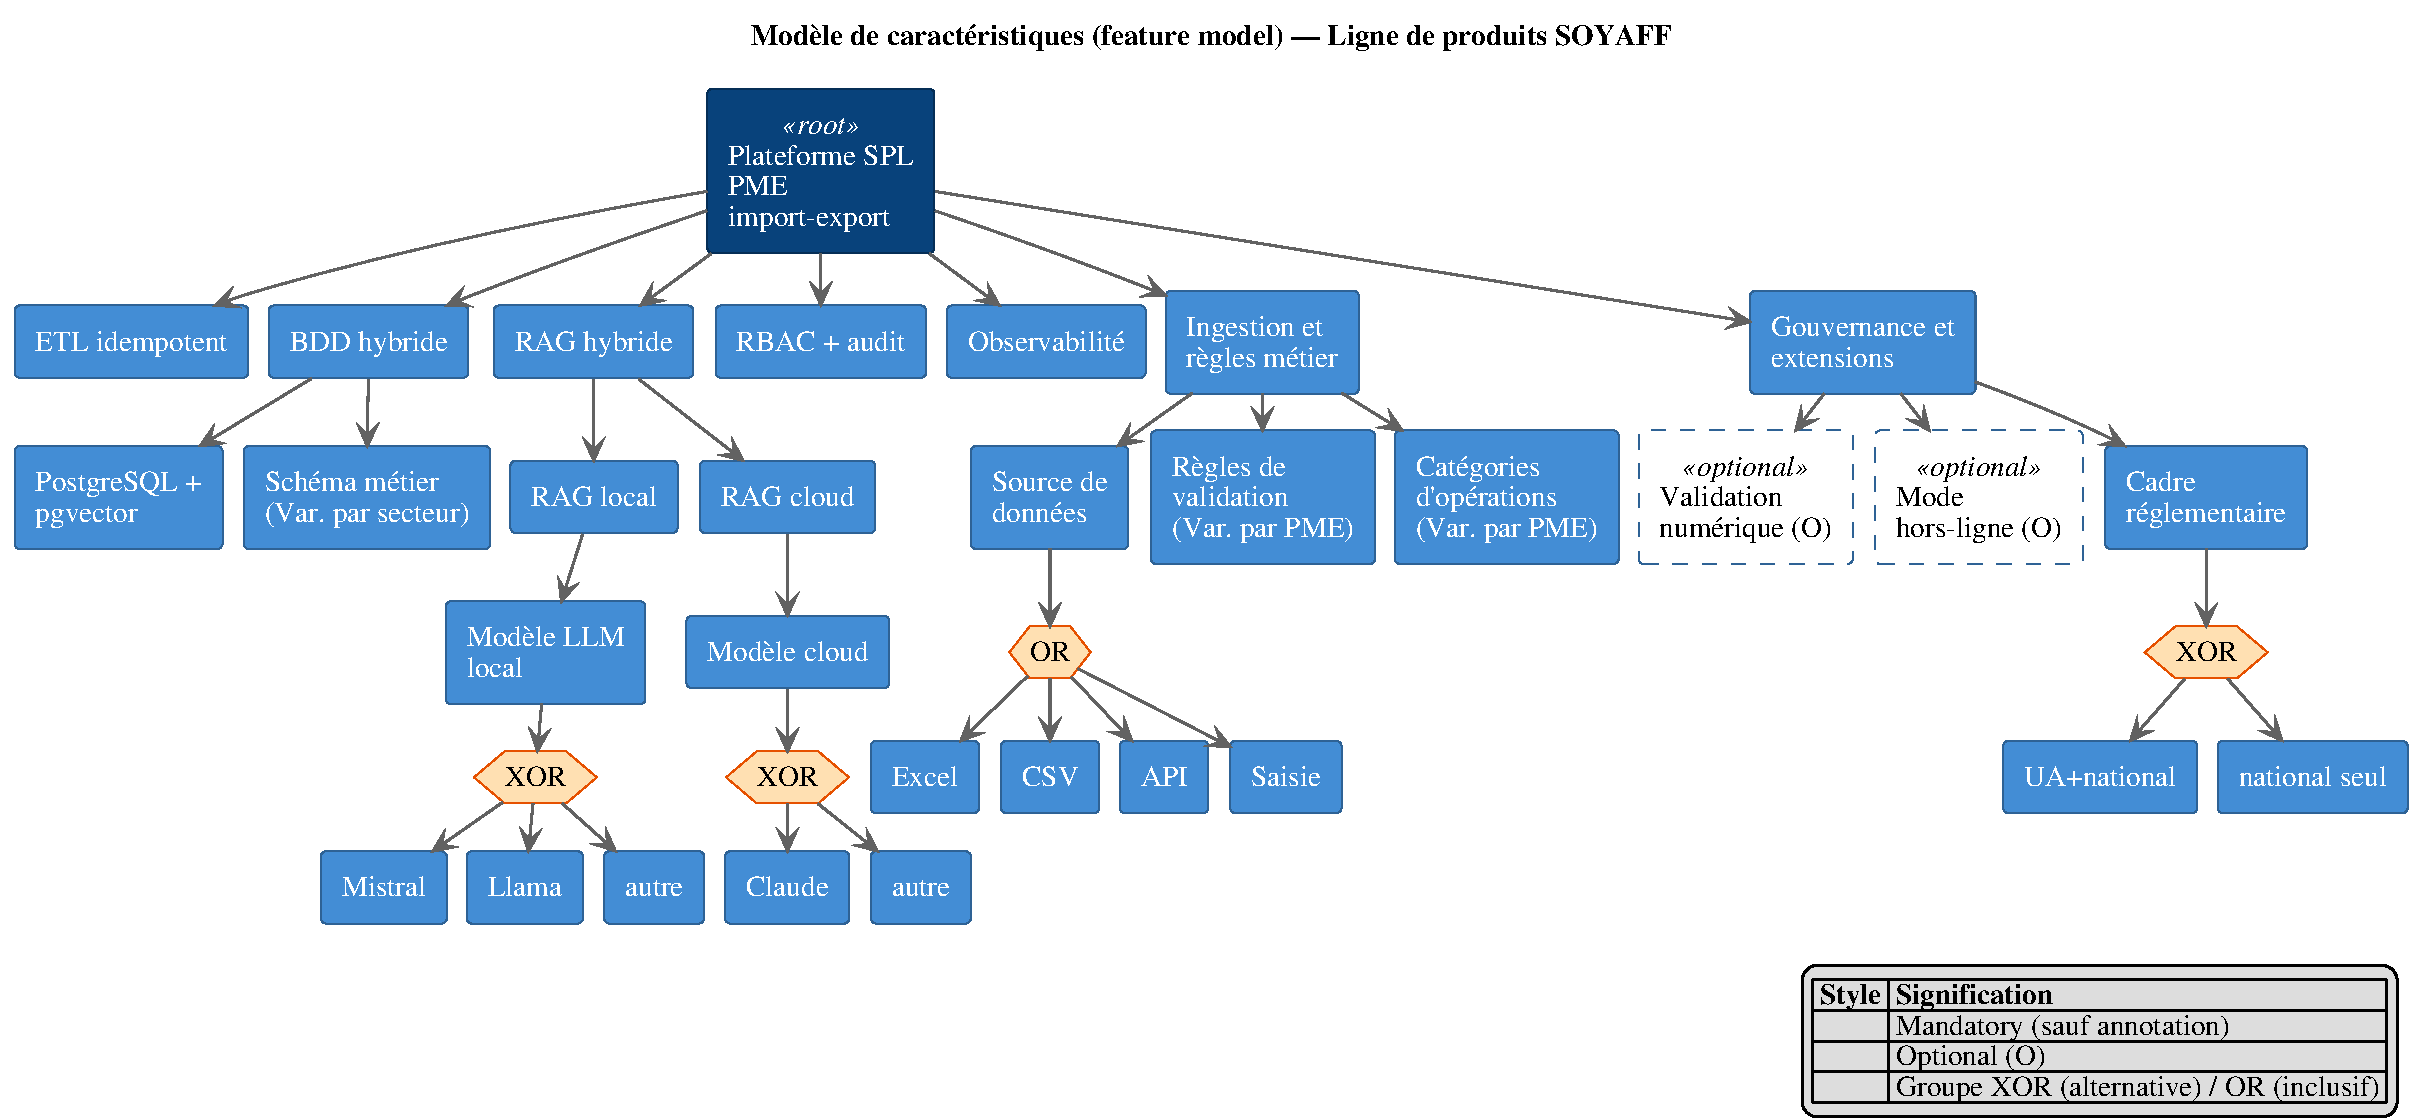
\includegraphics[width=\linewidth,height=0.85\textheight,keepaspectratio]{figures/fig_feature_model.pdf}
    \caption[Modèle de caractéristiques de la ligne de produits SOYAFF]{Modèle de caractéristiques (\textit{feature model}) de la ligne de produits SOYAFF. Sauf annotation contraire, une caractéristique est obligatoire.}
    \label{fig:feature_model_spl}
    \source{Schéma de l'auteur}
\end{figure}
\end{landscape}

Toutes les branches de premier niveau sont obligatoires. Trois d'entre elles (ETL idempotent, RBAC et audit, supervision) n'ont aucune variabilité. Les autres ne varient que dans leurs feuilles, jamais dans leur existence. C'est l'argument central pour H4 : la réutilisation est forte, et la variabilité est bornée à quelques points identifiés. Une contrainte n'apparaît pas dans l'arbre : le RAG local \emph{requiert} un moteur d'inférence local, donc le conteneur Ollama.

\subsection{Instanciation illustrative : SODRAF SARL (Bamako, Mali)}
\label{sec:spl_instanciation}

Pour rendre l'analyse concrète, nous dérivons sur le papier un second produit pour SODRAF SARL. Cette société de commerce d'import-export de produits alimentaires (riz, sucre, boissons), basée à Bamako, emploie de 51 à 200 personnes et est \textbf{partenaire commercial de SOYAFF} sur le corridor. Il s'agit d'une dérivation analytique, pas d'un déploiement.

\textbf{Ce qui est repris tel quel.} SODRAF gère elle aussi ses opérations sur des supports hétérogènes. Les six invariants sont repris sans modification : mêmes conteneurs, même topologie, même routage hybride.

\textbf{Ce qui est reconfiguré.}
\begin{itemize}
    \item \textbf{Le schéma métier.} Les camions, bons de livraison et chauffeurs laissent la place aux fournisseurs, produits, stocks et points de vente. C'est une modélisation de domaine à part entière, pas un paramétrage.
    \item \textbf{Le cadre juridique.} SODRAF relève du régime malien, hors Convention de Malabo : le socle juridique change de nature.
    \item \textbf{Les catégories et les règles métier.} Les catégories du transport (carburant, ration, frais de route) deviennent celles du commerce (achat, stockage, distribution, pertes) ; les contrôles de délai sont remplacés par des seuils de réapprovisionnement ou de péremption.
\end{itemize}

Aucun conteneur du plan applicatif, IA ou données (Tableau~\ref{tab:inventaire_conteneurs}) n'est remplacé ni supprimé. La charge réelle de reconfiguration du schéma n'a cependant pas été mesurée, et rien ne garantit qu'elle resterait contenue en pratique.

\subsection{Portée, limites et verdict sur H4}
\label{sec:spl_limites}

\textbf{Verdict.} L'architecture présente un noyau de six invariants et une variabilité bornée à sept points identifiés ; la dérivation vers SODRAF ne modifie aucun conteneur. \textbf{H4 est étayée analytiquement} : la réplicabilité est plausible sans refonte majeure. Elle n'est ni validée ni infirmée par l'expérience.

\textbf{Limites.}
\begin{itemize}
    \item \textbf{Un seul produit réel.} SOYAFF est le seul membre de la ligne construit et exploité ; SODRAF n'est dérivée que sur le papier.
    \item \textbf{Une variabilité en partie théorique.} Le modèle local est écrit en dur dans le code : le changer demande une modification du code, pas une simple configuration.
    \item \textbf{Le schéma métier reste le point le plus large.} Changer de secteur, même vers un secteur voisin, demande une nouvelle modélisation du domaine.
    \item \textbf{Le cadre juridique change de nature d'un pays à l'autre}, ce qui nuance l'idée d'une variabilité uniformément bornée.
\end{itemize}

La validation par un déploiement réel, chez SODRAF de préférence, est la suite logique de ce travail (section~\ref{chap:perspectives}).

\subsection{Synthèse et transition}
\label{sec:spl_synthese_transition}

H4 est étayée par l'analyse, pas encore démontrée par un second cas. Les quatre hypothèses ont maintenant été éprouvées : H2 par le benchmark, H1 et H3 par la mesure de l'impact, H4 par le raisonnement. Il reste à chiffrer le retour sur investissement (\S\ref{sec:roi}) et à répondre à la problématique (\S\ref{sec:reponse_problematique}).
